\subsection{Overview}

\subsection{Interface}

\subsection{Scheduling Engine}

\subsection{Agents}

The Agents are used to provide the Scheduling Engine as well as the programmer (through the \texttt{faust::resmon} API) with periodic informations about all participating systems that are relevant for scheduling descissions and job execution. \FAUST Agents are realized as independent command line applications that run on the execution hosts (usually on the head or gateway nodes) and report vital system and status informations like queue status, network load, filesystem availability, etc. back to a \FAUST application instance.

\begin{figure}[bth!]
  \begin{center}
    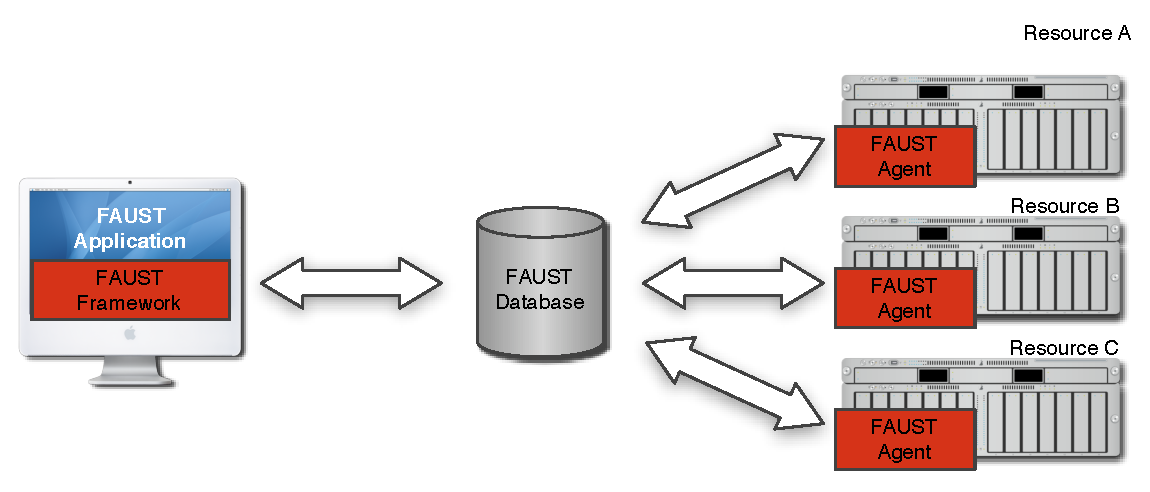
\includegraphics[width=0.95\textwidth]{figures/faust_agents_01}
    \caption{\label{fig:faust_agents_01} Example of a \FAUST application 
      instance running agents on three execution hosts. To ensure 
      application persitency, the communication between the application
      and the agents flows through a proxy database. }
  \end{center}
\end{figure}

Besides reporting system informations to the application, agents can optionally act as job submission endpoints. In this scenario, an application sends jobs directly to the agents for execution and not to the system's job service (like Globus, GridSAM, PBS, etc). This will usually happen, if the application scheduler (or the programmer) decides to apply 'hijacking' strategies like \textit{Glide-In} which require circumvention of local queueing systems.

\subsubsection{Database}

A critical design descission was that all communication between a \FAUST application and its agents must be routed through a proxy database to ensure global persitency in a distributed environment. This indirect communication between agents and application was motivated by two important requirements during the design process:

\begin{itemize}

\item{A \FAUST application must have the ability to disconnect and reconnect from its 
infrastructure whithout the need to abort and restart.}

\item{A \FAUST application might run in a restricted namespace (eg. firewalled). A 
communication proxy can help to avoid this restriction.}

\item{The data collected by the agents might be of interest to other application or
services. A central database allows other clients (Web-Services, etc.) to harvest
and use this data.}

\end{itemize}

The agents use the SAGA \textit{Advert Service} and its \textit{PostgreSQL}-based
middleware adaptor to read and write hierarchical entries from or to a centralized 
datbase. The structure of the database (as shown in Figure \ref?) is known to the 
agents and the application framework. In case the applications wants to read 
system informations from a certain agent, it simply reads the entries to which the
agent periodically writes its information. If the application framework wants to
send a command to an agent, it writes a command to the entry in which the agent
periodically looks for new commands.

Although the communication between agents and application is not very dense, this approach introduces a certain amount communication overhead that can slow down an application - especially with the current implementation of the \textit{PostgreSQL}-based SAGA middleware adaptor. A simple improvement would be the development of a high-performance SAGA Advert adaptor which would allow for higher data throughput without the need to change the 
\FAUST framework. Benchmarks for the current \textit{PostgreSQL}-based implementation
can be found in section \ref?.


\subsubsection{Mode of Operation}

The \FAUST Agents are transparently deployed and started by a \FAUST application as soon as a new \texttt{faust::service} object gets instantiated. Each \texttt{faust::service} instance is defined by a set of resources which represent possible target hosts for job submission. Each \texttt{faust::resource} has its own Agent for management, monitoring and information retreival. 

Unfortunately, different distributed infrastructures require different techniques to extract the informations that are required for effective scheduling. Although there are several more or less well defined interfaces to query these informations like \textit{NWS} or \textit{BQP}, it appears that in practice their existence and proper operation cannot be assumed. For this reason, agents require a relatively rich set of initial system informations that are used to generate subsequent runtime informations and performance predictions. Once deployed and started, an Agent follows the (simplified) execution scheme shown in Figure \ref{code:pseudo_agent} .

\begin{figure}[bth!]
\begin{alltt}
01   BEGIN
02    IF \emph{provided host description is usable on this machine} THEN
03      REPEAT
04         \emph{Gather informations and write to database}
05        IF \emph{Resource reservation request} THEN
06           \emph{Try to reserve resources through queueing system}
07        ENDIF
08        IF \emph{Job execution request} THEN
09          IF \emph{Resources available} THEN
10            \emph{Execute job}
11          ELSE
12             \emph{Report that no resources are available}
13          ENDIF
14        ENDIF
15      UNTIL  \emph{Termination request received}
16    ELSE 
17       \emph{Report error and terminate}
18    ENDIF
19   END
\end{alltt}
\caption{\label{code:pseudo_agent} Pseudocode describing the Agent's mode of
operation. }
\end{figure}

The agents provide basic logging and fault tolerance mechanisms which are crucial in a capricious distributed environment. 

\subsubsection{Host Files and Agent Repositories}


